This section aims to explore and analyze the key differences between Stratum V1 and Stratum V2, highlighting the advancements and improvements introduced by the latter. It will follow the public SV2 documentation from Braiins, summarizing the most interesting SV2 enhancements \cite{braiinsStratumNext}.\\

\noindent\textbf{Bandwidth consumption}

\begin{wrapfigure}{r}{0.6\textwidth}
    \centering
    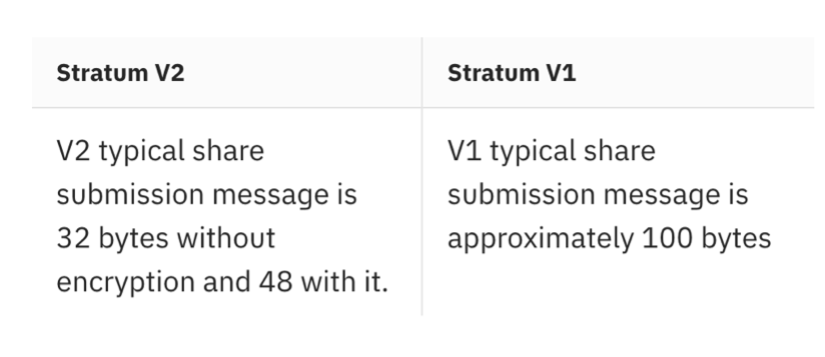
\includegraphics[width=0.6\textwidth]{Figures/sv2/sv2_5.png}
\end{wrapfigure}
\noindent The use of a binary protocol instead of a text-based one significantly reduces bandwidth usage.
In Stratum V1, making messages readable by humans resulted in some messages being unnecessarily large, approximately 2-3 times bigger than needed. 
However, in V2, these messages have been minimized to their essential size. Furthermore, V1 includes certain unnecessary messages like mining.subscribe, which have been eliminated in V2.\\

\noindent\textbf{Server CPU load}\\
Thanks to the introduction of standard and group channels, Stratum V2 achieves a reduction in server CPU load by implementing header-only mining for end devices (it will be explained later). This implies that the Merkle root, which was previously handled by end devices, is now always provided by an upstream node. Consequently, end devices are lighter since there's no need to perform any coinbase modifications. This simplifies the computational tasks for miners and, at the same time, significantly lightens the workload required for work validation (i.e. CPU load) on the server side.\\

\noindent\textbf{Header-only mining}\\
As anticipated in section \ref{sssec:sv2_hom}, Stratum V2 introduces the possibility for miners to open standard mining channels that don't permits coinbase transaction manipulation. In other words, end mining devices don't do any extranonce or Merkle path handling. This process if called \textbf{header-only mining}. The size of the search space for a device doing header-only mining for a particular value in the nTime field is $2^{NONCE\_BITS + VERSION\_ROLLING\_BITS}$ = 280Th, where NONCE\_BITS = 32 and VERSION\_ROLLING\_BITS = 16. This is a guaranteed search space before nTime rolling. The client that opens a particular standard channel owns the entire assigned search space and can split it further (e.g. between multiple hashing boards or individual chips) if necessary.\\

\noindent\textbf{Binary vs non-binary}\\
As described in \ref{sssec:sv2_framing}, SV2 has fixed message framing and it is precisely defined, which means that there isn't room for different interpretations of Stratum V2 like there was with V1. \\
Instead, Stratum V1 protocol relies on JSON, which has a sub-optimal ratio between the size of the message payload and the actual information transmitted. By transforming Stratum V2 into a binary protocol, the data efficiency significantly improves. This enhanced efficiency allows for the saved bandwidth to be allocated towards more frequent job submissions, thereby reducing hashrate variance.\\

\noindent\textbf{Job distribution latency}\label{sv2_jdl}

\begin{wrapfigure}{r}{0.6\textwidth}
    \centering
    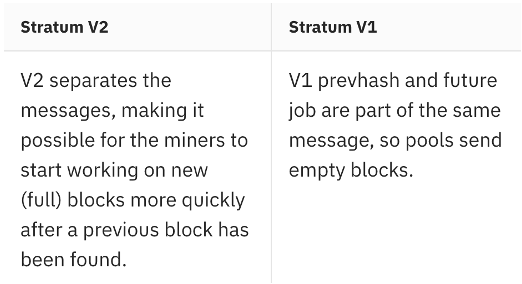
\includegraphics[width=0.5\textwidth]{Figures/sv2/sv2_6.png}
\end{wrapfigure}
\noindent In Stratum V1, mining pool servers send jobs to miners containing both the prevhash and Merkle root of the transaction lists to be included in the next block (this is done using the SV1 mining.notify message, as discussed in \ref{sssec:sv1_messages}).
So, these two pieces of data aren't separable, so there is a heavy (slow) data transfer necessary to distribute new jobs as soon as a new block (with a new prevhash) has been found and propagated. \\
In Stratum V2, it's possible to separate the prevhash from the rest of the predefined block data, which allows for the block data to be sent before a new prevhash is available. As a result, the new prevhash message can be sent on its own as soon as a valid block is found, and this transmission can occur much faster because the message doesn't include heavier data. This enables miners to begin working on new jobs more quickly than they could with Stratum V1.\\

\noindent\textbf{Man-in-the-middle attack prevention}\\
As analyzed at \ref{sssec:sv2:security}, Stratum V2 introduces a type of encryption scheme called AEAD (authenticated encryption with associated data) to address the security aspects of all communication that occurs between miners and pool servers. This provides both confidentiality and integrity for the ciphertexts (i.e. encrypted data) being transferred, as well as providing integrity for associated data which is not encrypted. Stratum V2 uses authenticated encryption with associated data (AEAD) so that possible adversaries will be unable to use share submission data to identify particular miners, thus maintaining the privacy of miners and protecting them against hashrate hijacking.\\

\noindent\textbf{Empty block mining elimination}\\
Very similarly to the \ref{sv2_jdl} point, the elimination of the incentive for empty block mining comes down to the separation of the prevhash message from other block header data. With Stratum V1, there is an incentive for pools to send empty blocks containing the new prevhash as soon as possible, as these messages will arrive faster than a message containing a full block. By separating these two messages in Stratum V2, it's now possible for pools to send full blocks to miners before the new prevhash message. In other words, the miners can be prepared to start working on a new (full) block before the previous block has been found, and then all they need is the new prevhash message to begin working on that next block. Since this prevhash message is the same size (i.e. takes the same amount of time to arrive) regardless of whether or not the pool has sent an empty block or a full block, there is no longer an incentive to mine on empty blocks.\\

\noindent\textbf{Job selection}\\
Job selection by end miners has been included as an optional component of Stratum V2, separate from the main mining protocol. 
The name Job 'Negotiation' Protocol is telling, as job selection is indeed a negotiation process between a miner and a pool. The miner proposes a block template, and it is up to a pool to accept or reject it. Once a negotiated template has been accepted, the results can be used by any number of mining devices, even hundreds of thousands of them. The reason this is separate from the main mining protocol is to allow pools to terminate connections on separate infrastructure from the main mining protocol, that way there is no impact on the efficiency of actual share submissions.\\

\noindent\textbf{Multiplexing}\\
In SV2, there can theoretically be as many as $2^{32}$ (around 4.3 billion) open channels within a single physical connection (e.g. TCP) to an upstream stratum node. These channels are independent and have unique channel IDs, meaning that many devices can simultaneously receive different job assignments using the same connection, saving on infrastructure costs. At the same time, the channels may all share some information for greater efficiency, such as when a new prevhash is broadcasted.\\

\noindent\textbf{Native version rolling}\\
Each Bitcoin block header contains a version field whose bits can be freely used to extend the search space for a miner. Rolling the version bits can greatly reduce the frequency with which new jobs need to be distributed, and it's already a common technology (BIP320, \href{https://en.bitcoin.it/wiki/BIP_0320}{https://en.bitcoin.it/wiki/BIP\_0320}). With SV2, version rolling becomes a native part of the mining protocol.\\\\\\


\noindent The features and improvements mentioned earlier are the main additions brought by the Stratum V2 protocol. They are taken from the protocol specifications released in 2019, as mentioned before. \\ 
In the next section, it will be explained the current implementations of the SV2 protocol specifications, including the birth of an independent development group, which is focused on standardizing a totally open source and community-based implementation, called SRI (Stratum Reference Implementation).